\documentclass{article}

\usepackage[T1]{fontenc}
\usepackage[utf8]{inputenc}
\usepackage{lmodern}

\usepackage{hyperref}
\usepackage{graphicx}

\usepackage{minted}

\begin{document}

\title{Boot with GRUB}
\author{Wayne Marshall in Linux Journal}
\date{Apr 30, 2001}

\maketitle

\begin{abstract}
Especially useful for multiboot, partitioned systems, GRUB offers flexibility and convenience for startup.
\end{abstract}

\section{Introduction}

GRUB: it's neither larva, fast food nor the loveliest of acronyms in the GNU herd of free software. Rather, GRUB is the GNU GRand Unified Bootloader. And, it is truly the greatest loader for booting Linux and practically any other OS — open source or otherwise — you may have scattered on your platters.

GRUB is independent of any particular operating system and may be thought of as a tiny, function-specific OS. The purpose of the GRUB kernel is to recognize filesystems and load boot images, and it provides both menu-driven and command-line interfaces to perform these functions. The command-line interface in particular is quite flexible and powerful, with command history and completion features familiar to users of the bash shell.

GRUB is in its element with the multiboot, multidisk systems typical of Linux and open-source adventurers who may simultaneously test or track several Linux distributions, the BSDs, GNU/Hurd, BeOS and perhaps that vestigial partition for Mr. Bill. Even if you stick with LILO as your system's primary boot loader, it's smart to keep a GRUB boot floppy handy as the best and fastest way to get your system back if you otherwise cream your master boot record (MBR). If you have done any number of multiboot installations, you know exactly what I'm talking about. Should you need any more reasons for considering GRUB, check out the sidebar, “Why GRUB”\marginpar{“Why GRUB” is in Section \ref{sec-why-grub}}. Let's get started!

\section{Installation}

Installation of GRUB is a two-step process. The first step is to install or build GRUB in a host OS environment, and for this we will, of course, use Linux. The second step is to install and configure GRUB as the boot loader for your system.

The first step is the usual: download the source archive, untar it, configure and make install. Assuming you have found a source mirror (see \href{www.gnu.org/software/grub/grub.html}{www.gnu.org/software/grub/grub.html}) and downloaded the source distribution into a suitable working directory, continue with:

\begin{minted}{bash}
    tar -xzvf grub-0.5.96.1.tar.gz
    cd grub-0.5.96.1
    ./configure
    make
    make install
\end{minted}

This should create the executables:
\texttt{grub}, \texttt{grub-install} and \texttt{mbchk};
install support files in \texttt{/usr/local/share/grub/i386-pc/},
and install the GNU information manual and man pages.

For the second step of installation, we will first build and work with a GRUB boot floppy. This way we can use GRUB to learn about its features while testing various configurations for our particular system. After getting comfortable with the GRUB setup on floppy, we will then install it onto the MBR of the system's first hard disk. Even if you decide not to install GRUB on your hard disk right away, no harm done: you will now have your own GRUB boot floppy available to rescue systems with trashed boot loaders.

\section{Preparing a GRUB floppy}

GRUB recognizes a number of different filesytem types,
including Linux \texttt{ext2fs}, \texttt{Reiser}, \texttt{MINIX}, BSD's \texttt{ffs}, as well as \texttt{FAT},
so it is possible to make a GRUB boot floppy with any of these filesystems. We will stick to \texttt{FAT} for this example, however, because it is the lowest common denominator, and most OSes have tools for mounting and reading/writing files on \texttt{FAT} floppies. That way, we will always be able to get to its menu configuration file if we need to.

Scrounge around in your junk drawer for some unused floppy (a new one would be even better), and give it a fresh format and \texttt{FAT} filesystem:

\begin{minted}{bash}
    fdformat /dev/fd0
    mkfs -t msdos /dev/fd0
\end{minted}

We are going to put some files on this disk, so go ahead and mount to your usual floppy mount point (here I use \texttt{/floppy}):

\begin{minted}{bash}
    mount -t msdos /dev/fd0 /floppy
\end{minted}

Now install the directories and files GRUB will need:

\begin{minted}{bash}
    mkdir -p /floppy/boot/grub
    cp /usr/local/share/grub/i386-pc/stage* /floppy/boot/grub
\end{minted}

The floppy can then be unmounted, \textbf{\texttt{umount /floppy}}, but leave it in the drive. The GRUB floppy is prepared and ready for the final installation, which is to install the GRUB boot loader in the MBR of the floppy itself. For that, we will use the grub executable we have built with our Linux installation. Start the executable at the Linux command prompt: \textbf{\texttt{grub}}.

This brings up an emulator of GRUB's command shell environment, which looks like Figure \ref{fig:comline}. We will discuss the features of this shell in more detail a little further on. For now, enter the following series of commands at the grub prompt:


\begin{minted}{bash}
    grub> root (fd0)
    grub> setup (fd0)
    grub> quit
\end{minted}

      \begin{figure}
      \centering
      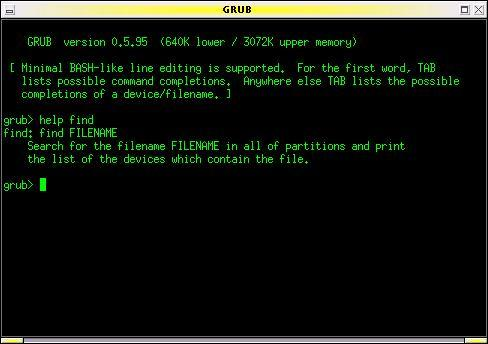
\includegraphics[width=0.8\linewidth]{Boot-with-GRUB_w768.jpg}
      \caption{GRUB in command-line mode. Note the on-line help}
      \label{fig:comline}
      \end{figure}

And that's it! This sequence of commands completes the installation of GRUB on the floppy disk. It is now bootable and will allow us to boot any other OS on our system.











\section{Demonstrating GRUB}

To see how GRUB may be used to boot a multitude of different operating systems, consider this example setup:

First Hard Disk (SCSI, Linux \texttt{/dev/sda}): 1st primary partition: Win98 2nd primary partition: Linux-Slackware 3rd primary partition: Linux-Debian 4th primary partition: Linux SwapSecond Hard Disk (SCSI, Linux \texttt{/dev/sdb}) 1st primary partition: FreeBSD 2nd primary partition: OpenBSD 3rd primary partition: BeOS

Note that although GRUB and Linux are capable of dealing with installations in extended partitions, here we show a preference for using primary partitions whenever possible. Filesystems in primary partitions are often mountable by other operating systems, whereas cross-OS mounting filesystems in extended partitions is often not supported.

This system has two hard disks with six different operating systems using seven partitions. As you probably know, each OS has its own nomenclature for naming devices and partitions.
For example, the Slackware installation would be known to Linux as \texttt{/dev/sda2} (with swap on \texttt{/dev/sda4}),
while FreeBSD would recognize its filesystem on \texttt{/dev/da1s1a}.
Alternatively, if the system were configured with IDE hard disks, Slackware would be on \texttt{/dev/hda2},
and FreeBSD would refer to its root directory on \texttt{/dev/ad1s1a}.
You get large helpings of this alphabet soup whenever maintaining any multiboot setup.

Since GRUB also needs to be capable of loading any of these systems, it has its own OS-neutral naming conventions for referring to devices.
Hard disks are all \texttt{hd},
floppy disks are \texttt{fd},
device numbering starts from zero, partition numbering starts from zero and complete device names are enclosed in parentheses.

With these naming rules, the floppy disk is \texttt{(fd0)},
the Win98 partition is \texttt{(hd0,0)},
and GRUB recognizes the Slackware and Debian partitions respectively
as \texttt{(hd0,1)} for slackware and \texttt{(hd0,2)} for debian.

The BSDs further subdivide their own partitions (or “slices” in BSD terms), and GRUB would refer to the root mount for the FreeBSD system on \texttt{(hd1,0,a)}.

Okay, ready to give GRUB a taste? Slide the GRUB floppy in the drive and reboot your system (with your system's BIOS configured to boot from \texttt{A:} drive). You should see GRUB's terse boot messages and then find yourself in the GRUB command-line environment as shown in \ref{fig:comline}.

To start, let's boot Slackware. Enter the following commands at the grub prompt:

\begin{minted}{bash}
    grub> root (hd0,1)
    grub> kernel /vmlinuz root=/dev/sda2 ro vga=791
    grub> boot
\end{minted}

Badda-bing, badda-boom, that postage-stamp-sized Tux appears in the upper-left corner of your screen (yes, Slackware is configured to use the framebuffer device), and Linux bootstraps its jolly way into glorious being.

Another example. Reboot the system again with the GRUB floppy, and enter the following commands at the grub prompt:

\begin{minted}{bash}
    grub> rootnoverify (hd0,0)
    grub> makeactive
    grub> chainloader +1
    grub> boot
\end{minted}

Now your screen turns into a vague blue cloud, and you think you have made some horrible mistake. Then you realize it's only Windows and you remind yourself to expunge this partition one day soon.

Let's take a closer look at these examples. In the Slackware boot, we first used the GRUB root command to specify the device for GRUB to access. If the device has a filesystem recognized by GRUB (that is, one of \texttt{ext2fs}, \texttt{reiser}, \texttt{ffs}, etc.), it attempts to mount it and get its partition information, then reports its success following the command. Thus, you would see the following command/response dialog on your screen:

\begin{minted}{bash}
    grub> root (hd0,1)
    Filesystem type is ext2fs, partition type 0x83
\end{minted}

Next, we used the GRUB kernel command to specify the boot image for GRUB to load.
The argument to the kernel command is the filename of the boot image
relative to the device specified by the root command above.
The kernel image file can also be specified in explicit \texttt{(device)/filename} terms as follows:

\begin{minted}{bash}
    grub> kernel (hd0,1)/vmlinuz
\end{minted}

The kernel command gives you great flexibility for specifying the boot image you wish to load.
For example, if we saved a previous version of a kernel to the file \texttt{/vmlinuz.old},
we could specify it with this command (which shows GRUB's response):

\begin{minted}{bash}
    grub> kernel /vmlinuz.old root=/dev/sda2 ro vga=ask
    [Linux-bzImage, setup=0xe00, size=0xfad30]
\end{minted}

The arguments following the name of the boot image are passed to the target kernel and aren't related to GRUB. For Linux, these kernel arguments are pretty much what you would specify them to be in \texttt{lilo.conf}.
In our example, we tell the kernel what device to mount for the root partition (\texttt{root=/dev/sda2 ro}), using the device nomenclature expected by Linux.
Note here that we also use the \texttt{ro} flag to mount the root filesystem read-only initially while it performs its filesystem check.
The other kernel argument in our example simply demonstrates setting another kernel variable (\texttt{vga=791}) to use a particular vga mode for the framebuffer display.

Finally, the last command is \textbf{\texttt{grub> boot}}. The kernel image specified is now loaded and sent rolling down the royal road to bootdom.

The second example, using Win98, demonstrates the use of GRUB's chain-loading mechanism. This method of booting loads the target OS's own boot-chain-loader rather than a kernel image of the OS. In this instance, we specified:

\begin{minted}{bash}
    grub> rootnoverify (hd0,0)
    grub> chainloader +1
\end{minted}

First, the \texttt{rootnoverify} command is for OS filesystems not specifically recognized by GRUB,
so that GRUB will not try to mount the partition.
Next, the \texttt{chainloader} command will use the first sector of the partition of device \texttt{(hd0,0)} and attempt to boot whatever it finds there.
This is a common means of booting OSes that install their own boot loaders in the first sector of the partition where they are installed (this is sometimes called the partition boot sector or PBR).

Finally, the \texttt{makeactive} command sets the active flag in the partition table for the device specified by the root command, as some operating systems, like Win98, require.

The GRUB command line is easy and fun, and you should boot the different OSes on your system a few times to get the hang of it. While you are testing, be sure to keep any notes specific to getting your particular kernels successfully loaded. This information will be useful later when you configure the menu system of GRUB to perform these command-line steps automatically.

But before we leave the command line, here are a few more GRUB commands to look at.

The help command will display a list of the 40 or so commands available in GRUB. Typing the name a particular command after help will produce on-line help for that particular command. So \textbf{\texttt{grub> help kernel}} will tell you all about using the kernel command.

The cat command can be used to view the contents of a file. For example, \textbf{\texttt{grub> cat (hd0,2)/etc/fstab}} will show the contents of the \texttt{/etc/fstab} file in the Debian installation. This is a very handy way of pulling out system configuration information if your normal boot loader gets whacked. Note also as you are using the GRUB command line that, like bash, up and down arrows will scroll through command history, and a tab will complete the name of a GRUB command or filename.

Finally, you can call up a specific menu interface with the configfile command as in:

\begin{minted}{bash}
    grub> configfile (fd0)/boot/grub/menu.lst
\end{minted}

This will switch GRUB into its menu mode with an interface defined by the file, menu.lst. We haven't created that file yet, but — look out, segue coming! — that's exactly what we will do next.


















\section{Menu Configuration}

Using the GRUB command line is cool, but after a few thousand system starts, you will probably get a little tired of entering the same commands at the GRUB prompt and long for something a little more automated. Good news from the GRUB gang: you get a fully configurable menu interface at no extra charge! The GRUB boot menu gives you point-and-shoot boot selection, unattended default boot after a configurable timeout, any number of fallback boots if previous boots fail, toggle between command-line and menu modes, and interactive editing of menu selections and password protection. These features give GRUB an ease of use to match its tremendous functionality.

When GRUB boots, it automatically looks for the \texttt{/boot/grub/menu.lst} file on its boot device (the last three letters are “ELL ess tee” and not “one ess tee”). If the file is found, GRUB automatically enters its menu mode and presents the user with a stunning interface, as shown in \ref{fig:menu}.

      \begin{figure}
      \centering
      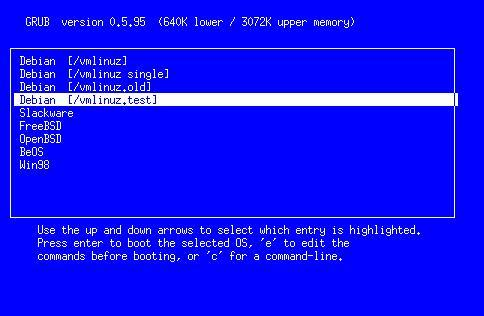
\includegraphics[width=0.8\linewidth]{Boot-with-GRUB_w768_GRUB-menu.jpg}
      \caption{GRUB's Boot Menu Interface}
      \label{fig:menu}
      \end{figure}

Listing 1
[found at \href{ftp://ftp.linuxjournal.com/pub/lj/listings/issue85/}{LJ's web site}]
\marginpar{Listing 1 is in Appendix \ref{list-1}}
shows the configuration file responsible for this demonstration menu. As you can see, it is a simple text file typical of many UNIX configuration files, where lines starting with hashes (\texttt{\#}) and blank lines are ignored.


The first set of commands sets general configuration variables. The \texttt{timeout} command sets the time in seconds to wait for the user to make a selection before proceeding automatically to the default boot. The default command sets which of the following boot stanzas GRUB should attempt to boot automatically. Boot stanzas are numbered implicitly, starting from zero, according to their order of appearance in the configuration file. This order is also how they will be listed in the menu.

The fallback command specifies which of the boot stanzas to load if the default should fail. It is possible to set more than one fallback, as is shown in the example.

The color command lets you breathe a bit of life into the text-mode menu screen. The syntax for the color command is

\begin{minted}{bash}
    color  foreground/background  [ hilite-fg/hilite-bg ]
\end{minted}

where each of the \texttt{foreground/background} colors is specified with a name from the set of \texttt{black}, \texttt{blue}, \texttt{green}, \texttt{cyan}, \texttt{red}, \texttt{magenta}, \texttt{brown} and \texttt{light-gray};
\texttt{dark-gray}, \texttt{light-blue}, \texttt{light-green}, \texttt{light-cyan}, \texttt{light-cyan}, \texttt{light-red}, \texttt{light-magenta}, \texttt{yellow} and \texttt{white}.
Among these colors, only the first eight are used for the background.
The optional highlight color pair, if specified, will be used to show the current menu selection.
When not specified, GRUB will use the inverse of the normal colors.

The rest of the configuration file consists of the boot stanzas for our demonstration system. The title command marks the beginning of a new boot stanza, and its argument is the label that will be displayed for its entry in the menu, from the first non-white-space character to the end of the line. The remaining commands in each stanza are identical to those used when working from the GRUB command line. The exception here is that we no longer need to give a boot command; GRUB does this job without asking.

This example configuration gives only a sample of the many flexible uses of the GRUB boot loader. Besides multiple OSes, you can use GRUB to set up menu selections for test kernels, rescue kernels, different kernel options and so on.

All in all, the GRUB configuration file will be very similar to your \texttt{/etc/lilo.conf}. And after working with the GRUB command line and these examples, it should be a simple matter of firing up your favorite text editor and creating a menu configuration file suitable for your own system and preferences. Don't worry if it's not perfect the first time; you will see that you can make changes interactively, and the GRUB command line is always available as a fallback.

Once you've got your configuration file, mount your GRUB floppy again, and copy the file (say it has been saved as \texttt{mygrub.conf}) into the magic location:

\begin{minted}{bash}
    cp  mygrub.conf /floppy/boot/grub/menu.lst
\end{minted}

Now when you boot with your GRUB floppy — presto! — you will be greeted with a lovely boot menu like the one in \ref{fig:menu}. If you like, just stare at it for the few seconds it needs to count down from the timeout setting, and then it will automatically boot into your default OS. Or, use the arrow keys to highlight the OS you want to load and press return.
Or, type \texttt{c} to go to the now-familiar GRUB command prompt.
From the command prompt, press \texttt{ESC} to go back to the boot menu again.

It is also possible to edit the entries displayed in the menu.
Typing \texttt{e} will open a simple \texttt{vi}-like editor interface for the highlighted entry.
This allows you to adjust or add any settings to the configuration before booting.
Any changes made here will then remain in effect for the duration of the GRUB session.
To make permanent changes, you will later need to edit the configuration file on the boot disk,
saving the changes with your text editor.

Play with your GRUB floppy configuration until you have it set up the way you like.
After just a few system boots, you'll be slinging through GRUB like hashbrowns in a diner.








\section{Hard Disk Installation}

By this time you may be thinking, “Okay, GRUB has got it goin' on. But do I have to keep booting from this lame floppy all the time?” Of course not. Booting from floppy is for weenies.

The operation for installing GRUB on the master boot record of your hard disk is similar to the creation of a GRUB floppy. The one difference is that our floppy has all the resources GRUB needs in one place. That is, the boot image, support and configuration files are all on the floppy device MBR and \texttt{/boot/grub/} directory. In a hard disk setup, you can choose where you want these resources to be.

For example, you could set up a \texttt{/boot/grub} directory on the first partition of your first hard disk and copy all GRUB's files into it as we did in our floppy setup. In our demonstration system, this would be the Win98 partition, and you may choose to do it that way if you want.
But you can also set up the \texttt{/boot/grub} directory up in any \texttt{device/partition}
on your machine with a filesystem supported by GRUB.
In practice it is usually best to install this support directory in your most frequently used and/or most stable partition; that is, one that you aren't reinstalling all the time.

For this example, we will use the Slackware partition since this stays pretty stable,
and I tend to do more tracking and installations in the Debian system. 
Once this decision is made, everything else is simple.
First, boot into Slackware, create the \texttt{/boot/grub} directory
and copy GRUB's files into it
(these are all the files that the GRUB build installed
in the \texttt{/usr/local/share/grub/i386-pc} directory).
Make sure to put your handcrafted \texttt{menu.lst} configuration file in here, too.

Next, start GRUB, either with the grub executable you built in Linux or by rebooting with the GRUB floppy. If GRUB starts in menu mode, press c to go to command-line mode. Enter the following commands at the grub prompt:

\begin{minted}{bash}
    grub> root (hd0,1)
    grub> setup (hd0)
    grub> quit
\end{minted}

You're done. Your system is now fully GRUB'd, installed in the MBR of your hard disk. Type \textbf{reboot} as root (or take the floppy out and jab the keyboard with the old three-prong) and watch just how fast GRUB comes up now!

A few words of explanation about these installation commands.
The first, \texttt{root (hd0,1)},
tells GRUB to mount this device,
in this case the partition with the Slackware installation.
All files will now be relative to this device,
so the GRUB installer will know to look for its support files
in the \texttt{\texttt{/boot/grub}} directory we created in the Slackware partition.

The second command, \texttt{setup (hd0)}, is a simplified front end to GRUB's install command. Note in particular that we specify the device as \texttt{(hd0)} and not \texttt{(hd0,0)}. Device \texttt{(hd0)} results in GRUB's installation to the master boot record, which is what we want. If we had instead used \texttt{(hd0,0)}, GRUB would be installed to the boot sector of the first partition, rather than the MBR. The difference is crucial; your technical writer makes mistakes like this so you don't have to. While each partition can have a boot sector, your hard disk will have only one master boot record the BIOS loads every time you start your machine. Unless you are doing some kind of funky boot-chaining, like using LILO to boot GRUB, you will usually want to install GRUB in the master boot record.

When GRUB installs itself on a device, it first copies a small piece of itself to the MBR, which it calls stage1. Then it follows stage1 with just enough information about where to find the rest of GRUB. In our example, GRUB will put stage1 in the MBR, followed by a blocklist that points to the Slackware partition. GRUB will then find the rest of what it needs (its stage2 files) in the \texttt{/boot/grub} directory.

To check this setup, just edit the menu configuration file
in Slackware's \texttt{/boot/grub/menu.lst} at any time.
Any changes will be reflected in the next boot.

\section{Error Recovery}

If you should foul up the hard disk installation somehow or want to uninstall GRUB from your system, here's what you need to know.

First, if you ever want to clean your MBR from whatever is installed there, the canonical method is to use the \texttt{fdisk} program from an MS-DOS boot floppy:

\begin{minted}{bash}
    A:> FDISK /MBR
\end{minted}

Of course, this isn't necessary if you just want to go back to LILO as your system's boot manager. In that case, simply make sure your \texttt{/etc/lilo.conf} file has a line that reads \textbf{\texttt{boot=/dev/hda}}. Then, when the rest of the \texttt{lilo.conf} file is the way you want, just rerun LILO. This will put LILO back on the MBR of your system.

If you install GRUB in the boot sector of a partition, instead of the MBR (such as specifying \texttt{setup (hd0,0)} instead of \texttt{setup (hd0)}), you may need to reinstall that OS's boot loader. In the case of DOS/Windows, this means running the sys command from your DOS/Windows boot floppy: \textbf{\texttt{A:> SYS C:}}.

If, this is a Linux partition, it is again effective to rerun LILO, where \texttt{/etc/lilo.conf} has a line in the boot stanza that reads \textbf{\texttt{root=/dev/hda1}}.

In general, most OSes will have a way to reinstall their partition's boot sector without doing a full reinstallation from scratch. (For FreeBSD, see \texttt{boot0cfg(8)}; for OpenBSD, see \texttt{installboot(8)}.)

In practice, especially if you followed through on the GRUB floppy examples, you should find that GRUB itself is one of the best rescue and system recovery tools in your toolkit. For example, if you have ever made a screwup in your \texttt{lilo.conf} file, you know you can be in for some major pain if your system won't boot. With GRUB, you always have a miniature, self-contained operating system that can recognize and mount different filesystems, find files, locate kernels and boot them, bringing your system back to life so you can work on it. At times like these, GRUB can save your bacon.













\section{Conclusions}

As is typical of GNU software, GRUB is rich with capabilities beyond what are described here. Some of these include:

\begin{itemize}
    \item Remapping disks and partition hiding, so you can even run multiple versions of DOS/Windows, on other than the first hard disk.
    \item Network booting with BOOTP and DHCP protocols, to support multiboot schemes across a network and diskless operation.
    \item Keyboard remapping, disk geometry access, memory reading, I/O port and processor probes, password protection, decompression support, etc.
\end{itemize}

See the GNU information manual for more information on these topics. GRUB is under active development, and even more features are planned for future releases.

In this brave GNU world, with vast acreage of cheap hard disk and a glut of great free OSes available, you really need a flexible and user-friendly boot loader to manage them all. Grab GRUB and give it a go.

\section{Why GRUB?}
\label{sec-why-grub}

Quite a few boot managers are available. Of course, Linux uses LILO, FreeBSD installs BootEasy, and you can also use OS-BS, payware like System Commander and other boot managers that ship with commercial operating systems like OS/2 and NT. So why GRUB?

OS-neutral: GRUB is not tied to any particular platform, and you don't need to run any special operating system to install and configure it. With LILO, for example, you need to be able to get into a Linux system for setup and maintenance, and remember to run the LILO binary after changing \texttt{/etc/lilo.conf}. GRUB can be set up and maintained from a number of systems, and any changes to its configuration file are immediately available.

Interactive: GRUB offers an interactive and configurable menu interface, and a command-line mode is always available. The command-line features are invaluable for getting into an OS whose boot configuration got creamed. Even boot settings within menu items can be interactively adjusted as necessary from within a GRUB session.

Powerful: If your BIOS handles LBA mode, GRUB can boot kernels beyond the 1024th cylinder, making kernel installations possible in partitions beyond 8GB. GRUB can do tricks with disk mapping and partition hiding, so you can run most OSes from whatever disk you want. GRUB also has network boot capabilities, enabling BOOTP and DHCP from remote servers.

GRUB is actively maintained and under continuing development. Its acronym expresses the goals of its authors to become the unified bootloader, so that every new OS project need not invent its own boot system. Although GRUB is primarily available for i386 systems, ports are underway and in various stages of completion for other architectures as well. By learning to use GRUB, you can be confident in having a single boot manager to handle any OS you may ever choose to install.









\section{Author}

\begin{minipage}{0.3\textwidth}
    
\includegraphics{author-photo_Wayne.jpg}
\end{minipage}
\begin{minipage}{0.5\textwidth}
    Wayne Marshall (guinix@yahoo.com) is a UNIX programmer
    and technical consultant currently living in Guinea, West Africa.
    When not grubbing about with computers,
    he enjoys taking the pirogue for day trips to
    the local islands near Conakry with his wife, Paula.
\end{minipage}











\clearpage
\appendix

\section{Listing 1}
\label{list-1}

Listing 1. \texttt{/boot/grub/menu.lst}

\begin{minted}{bash}
# /boot/grub/menu.lst
# grub boot menu configuration

# general configuration:
timeout  10
default   0
fallback  2
fallback  4
color     light-gray/blue  red/light-gray

# boot stanzas follow
# each is implicitly numbered from 0
# in the order of appearance below

# (0) Debian (default boot):
title  Debian  [/vmlinuz]
root   (hd0,2)
kernel /vmlinuz root=/dev/sda3 ro

# (1) Debian - runlevel 1
title  Debian  [/vmlinuz single]
root   (hd0,2)
kernel /vmlinuz single root=/dev/sda3 ro

# (2) Debian-old (first fallback)
title  Debian  [/vmlinuz.old]
root   (hd0,2)
kernel /vmlinuz.old root=/dev/sda3 ro

# (3) Debian-kernel testing
title  Debian  [/vmlinuz.test]
root   (hd0,2)
kernel /vmlinuz.test root=/dev/sda3 ro

# (4) Slackware (second fallback):
title  Slackware
root   (hd0,1)
kernel /vmlinuz root=/dev/sdb2 ro vga=791 mem=256M

# (5) FreeBSD:
title  FreeBSD
root   (hd1,0,a)
kernel /boot/loader

# (6) OpenBSD:
title  OpenBSD
# You would like to use:
##root   (hd1,1,a)
##kernel --type=openbsd /bsd
# But openbsd passes bios & kernel parameters with
# its own bootloader, the first stage of which is
# installed in the partition boot record, and in
# turn calls /boot, which in turn loads kernel /bsd.
# So just use the GRUB chainloader instead:
root (hd1,1)
makeactive
chainloader +1

# (7) BeOS:
title  BeOS
rootnoverify  (hd1,2)
makeactive
chainloader +1

# (8) WinDoze
title Win98
root  (hd0,0)
makeactive
chainloader +1

# end file menu.lst

\end{minted}



\end{document}
